\documentclass[12pt]{article}

\usepackage{fancyhdr}
\usepackage{geometry}
\usepackage[utf8]{inputenc}
\usepackage[T1]{fontenc}
\usepackage[ngerman]{babel}
\usepackage{amsmath,amssymb,amstext}
\usepackage{hyperref}
\usepackage{cancel}
\usepackage{dsfont}
\usepackage{physics}
\usepackage{lmodern}
\usepackage{enumerate}
\usepackage{enumitem}
\usepackage{graphicx}
\usepackage{listings, color}
\usepackage[labelfont=bf]{caption}
\usepackage{titling}
\usepackage{siunitx}
\usepackage{tikz}
\usepackage{icomma}
\usepackage{revsymb}

\usepackage[backend=biber,backref=false,style=numeric-comp, sorting=none,block=ragged,firstinits=true]{biblatex}

\lstset{basicstyle=\scriptsize,breaklines=true} %Quellcode mit Umlauten und ganz klein
\lstset{literate=
	{Ö}{{\"O}}1
	{Ä}{{\"A}}1
	{Ü}{{\"U}}1
	{ß}{{\ss}}2
	{ü}{{\"u}}1
	{ä}{{\"a}}1
	{ö}{{\"o}}1
}


%Geometrie----------------------------------------------------------------------------------------------------------

\geometry{a4paper, top=25mm, left=15mm, right=15mm, bottom=25mm,headsep=10mm, footskip=10mm}
\pagestyle{fancy}
\setlength{\parindent}{0pt} %Zeileneinrückung

\fancyhf{} %Setzt voreingestellte Kopf-und Fußzeilen-Eigenschaften zurück

\lhead{\nouppercase{\leftmark}}
\chead{}
\rhead{\thepage}

\lfoot{}
\cfoot{}
\rfoot{}

\title{\vspace{0cm}{\Huge Fortgeschrittenen-Praktikum II:\\ \vspace{1cm} Mößbauer-Effekt}}
\author{Saskia Bondza\\Simon Stephan}
\date{durchgeführt vom 20.02.2017 bis 24.02.2017}

\pretitle{%
	\begin{center}
		\LARGE
		
\includegraphics[width=6cm,]{../figures/siegel}\\[\bigskipamount]
	}
	\posttitle{\end{center}}

%neue Commands----------------------------------------------------------------------------------------------------------
\newcommand{\nab}{\vec{\nabla}} %direkter Befehl mit Vektorpfeil
\newcommand{\gra}[3][0.7]{
	\begin{minipage}[h!]{\textwidth}
		\centering
		\includegraphics[width=#1\textwidth]{../figures/#2.png}
		\captionof{figure}{#3}
	\end{minipage}
	\vskip 30 pt
}
\newcommand{\graX}[4][0.7]{
	\begin{minipage}[h!]{\textwidth}
		\centering
		\includegraphics[width=#1\textwidth]{../figures/#2.png}
		\captionof{figure}[#3]{#4}
	\end{minipage}
	\vskip 30 pt
}
\newcommand{\graTwo}[4][0.49]{
	\begin{minipage}[h!]{\textwidth}
		\centering
		\includegraphics[width=#1\textwidth]{../figures/#2.png}
		\includegraphics[width=#1\textwidth]{../figures/#3.png}
		\captionof{figure}{#4}
	\end{minipage}
	\vskip 30 pt
}
\newcommand{\graTwoB}[5]{
	\begin{minipage}[h!]{\textwidth}
		\centering
		\includegraphics[width=#1\textwidth]{../figures/#3.png}
		\includegraphics[width=#2\textwidth]{../figures/#4.png}
		\captionof{figure}{#5}
	\end{minipage}
	\vskip 30 pt
}
\newcommand{\del}[2][]{\frac{\partial #1}{\partial #2}}
\newcommand{\code}[1]{\texttt{#1}}

\addbibresource{fp_refs.bib}

%Titel,Inhalt----------------------------------------------------------------------------------------------------------

\begin{document}
	\pagenumbering{gobble} %verstecke Seitenzahl
	\maketitle
	\newpage
	

	
	\section*{Übersicht}

Mit Hilfe des Mößbauereffekts lässt sich eine sehr genaue und hochauflösende Aufnahme von Energiespektren durchführen. Der Mößbauereffekt beschreibt die rückstoßfreie Absorption und Emission von Photonen und wird in diesem Versuch zur Untersuchung der Emissionslinien des $14,4\,\si{keV}$-Zustands von $^{57}Fe$ verwendet. Dabei wird die Lebensdauer des Zustands auf zwei unterschiedliche Arten bestimmt und die Hyperfeinaufspaltung von Natureisen vermessen.\\

Für die Lebensdauer des $14,4\,\si{keV}$-Zustands von $^{57}Fe$ ergeben sich dabei folgende Ergebnisse:
\begin{align*}
	\tau_1&=(110\pm70)\,\si{ns}\\
	\tau_2&=(162\pm12)\,\si{ns}\\
	\tau_\text{lit}&=141\,\si{ns}\text{.}
\end{align*}

Aus der Hyperfeinaufspaltung des Natureisens wird das magnetische Moment des Kerns und das Magnetfeld am Kernort bestimmt. Diese ergeben sich zu:
\begin{align*}
	\mu_a&=(-0,157\pm0,004)\,\mu_N\\
	\mu_\text{lit}&=(-0,15531\pm0,00004)\,\mu_N\\
	B&=(32,9\pm0,3)\,\si{T}\\
	B_\text{lit}&=(33,3\pm0,1)\,\si{T}\text{ .}
\end{align*}
	
	\newpage
	
	\thispagestyle{empty}
	\tableofcontents
	\newpage
	
	%Schreiben----------------------------------------------------------------------------------------------------------
	\pagenumbering{arabic}
	
	\section{Einleitung}
	
Der Mößbauereffekt beschreibt die rückstoßfreie Resonanzabsorption von Kernzuständen. Da bei diesem Prozess die Energieverluste eliminiert werden, die bisher häufig ein Hindernis darstellten und zugleich eine sehr hohe Auflösung und Genauigkeit erreicht werden kann, bot diese Entdeckung zahlreiche Anwendungen. Ein klassisches Beispiel ist hier die Spektroskopie. Es konnte mit Hilfe des Mößbauereffekts aber auch die Energieverschiebung von Photonen im Gravitationsfeld der Erde $\frac{\Delta E }{E} = 10^{-16} $ pro Meter nachgewiesen werden, die von der Allgemeinen Relativitätstheorie vorhergesagt wird. Sogenannte MIMOS\footnote{\textbf{MI}niaturized \textbf{MO}essbauer \textbf Spektrometer} werden in Marssonden zur Analyse von Marsgestein verwendet.
Für die Entdeckung des nach ihm benannten Mößbauereffekts wurde Rudolf Mößbauer im Jahr 1961 der Nobelpreis verliehen.\\

In diesem Versuch sollen Absorptionslinien im Einlinien-Absorber Edelstahl und im Sechslinien-Absorber Eisen gemessen werden und deren Lebensdauer bestimmt werden. $^{57}$Fe weist eine sehr schmale Linie bei einer Energie von $14,4\,\mathrm{keV}$ auf.
Zur Messung dieses Übergangs wird der Absorber auf einem beweglichen Schlitten, der sich mit Geschwindigkeiten im Bereich von wenigen $\si{\frac{mm}{s}}$ bewegt, von einer $^{57}$Co-Probe bestrahlt, in der durch den Zerfall von Cobalt in einen angeregten Zustand von $^{57}$Fe, der wiederum in den Grundzustand zerfällt, ein Photon der Energie $14,4\,\mathrm{keV}$ abgestrahlt wird. Ein Detektor bestehend aus Szintillator und Photomultiplier hinter dem Absorber nimmt die Zählrate in Abhängigkeit der Geschwindigkeit auf. Im so entstehenden Spektrum erwarten wir den typischen Mößbauerpeak zu sehen, aus dem die Lebensdauer des angeregten Zustands bestimmt werden kann, sowie aus der Verschiebung zur theoretischen Resonanzfrequenz die Isomerieverschiebung. Für Natureisen kann aus der Hyperfeinaufspaltung, die Grund für die sechs Absorptionslinien ist, das magnetische Feld bestimmt werden. Außerdem werden verschiedene Messungen zur Bestimmung des Untergrunds durchgeführt.
Der in diesem Versuch untersuchte Übergang wurde bereits im Versuch "`Kurze Halbwertszeiten"' mit der Methode der verzögerten Koinzidenzen gemessen. 



	\newpage
	\section{Theoretische Grundlagen}

\subsection{Wechselwirkung von Photonen mit Materie}

Um $\gamma$-Strahlung detektieren zu können, muss die $\gamma$-Strahlung mit Materie wechselwirken. Wir unterscheiden dabei grundsätzlich drei Prozesse: Den Photoeffekt, den Compton-Effekt und die Paarbildung. In Materie klingt die Intensität von $\gamma$-Strahlung exponentiell ab:
\begin{align}
I&= I_0\cdot e^{-\mu x}
&\text{mit } 
\mu &= \mu_\text{photo} + \mu_\text{Compton} + \mu_\text{Paar}
\end{align}

Die einzelnen Prozesse werden im Folgenden erklärt.\cite{demtroeder}

\begin{itemize}
\item \textbf{Photo-Effekt}
Beim Photo-Effekt dringt ein Photon in das Atom ein und überträgt seine gesamte Energie an ein Elektron der inneren Schalen. Dabei wird Energie auf dieses Elektron übertragen, es wird aus der Atomhülle befreit und erhält kinetische Energie. Die hier entstandene Lücke wird über Abstrahlung eines $\gamma$-Quants oder eines Elektrons wieder gefüllt.

\item\textbf{Compton-Effekt}
Beim Compton-Effekt trifft ein einfallendes $\gamma$-Quant auf ein freies oder nur leicht gebundenes Elektron und überträgt einen Teil seiner Energie auf dieses. Dieser Prozess findet meist bei Energien zwischen $200\,\si{keV}$ und $5\,\si{MeV}$ statt.

\item\textbf{Paarbildung und Paarvernichtung \label{PVN1}}
Bei der Paarbildung entsteht durch die Wechselwirkung des $\gamma$-Quants mit dem elektromagnetischen Feld des Atomkerns oder eines Elektrons ein Teilchen-Antiteilchen-Paar, z.B. ein Elektronen-Positronen-Paar. Paarbildung ist für Energien über $1,022\,\si{MeV}$ möglich. Die über diesen Grenzwert hinausgehende Energie wird auf die entstandenen Teilchen übertragen, der Impuls wird vom Kern aufgenommen. Da das Positron nicht lange alleine existieren kann, vereinigt es sich unter Abstrahlung von zwei $\gamma$-Quanten mit einer Energie von je $511\,\si{keV}$ mit einem Elektron.
\end{itemize}

 \subsection{Nachweis der $\gamma$-Strahlung mithilfe des Szintillationszählers}
 Die emittierten Photonen müssen nun detektiert und ihre Energie bestimmt werden. Dazu wird ein Energie-sensitiver Detektor, eine Kombination aus Szintillator und Photomultiplier, verwendet.
 \paragraph{Szintillator} Ein Szintillator detektiert Teilchen eines bestimmten Energiebereichs. Es gibt organische und anorganische Szintillatoren, wobei in diesem Versuch ein anorganischer NaI(Tl)-Szintillator verwendet werden. Dieser besteht aus einem mit Thallium dotierten NaI-Kristall, in welchem die eintreffenden Photonen ihre Energie durch den Photo- oder Compton-Effekt an Elektronen abgeben. Je höher die Energie der Photonen ist, desto mehr Elektronen werden erzeugt. Diese Elektronen werden nun angeregt und später unter Emission  niederenergetischer Photonen wieder abgeregt. Die Dotierung mit Thallium verhindert, dass die emittierten Elektronen wieder absorbiert werden. Die Bandstruktur, auf der die Funktionsweise eines Szintillators beruht, ist in Abbildung \ref{Szinti} dargestellt.\cite{szinti}
 
 \graX[0.7]{Szinti}{Funktionsweise eines Szintillators}{Funktionsweise eines Szintillators \label{Szinti} \cite{szinti}}
 \paragraph{Photomultiplier}
 Das Licht wird nun vom Szintillator über Lichtleiter zum Photomultiplier geleitet. Dieser wandelt die Lichtimpulse des Szintillators durch den Photoeffekt in elektrische Impulse um, welche proportional zur Lichtintensität sind und verstärkt diese durch Elektronenvervielfachung. Die Funktionsweise eines Photomultipliers ist in Abbildung \ref{Multi} dargestellt.\cite{PM}
 
 \graX{photomult}{Funktionsweise eines Photomultipliers}{Funktionsweise eines Photomultipliers \label{Multi} \cite{PM}}

\subsection{Zerfallsschema von Cobalt}

Das in diesem Versuch verwendete $^{57}$Co zerfällt mit einer Wahrscheinlichkeit von $99,8\%$ und einer Halbwertszeit von $270$ Tagen über Elektroneneinfang in einen angeregten Zustand von $^{57}\mathrm{Fe}^*$ (siehe Abbildung \ref{Co57}):

\[ ^{57}_{27}\mathrm{\textbf{Co}} +\ \mathrm{e}^-\ \longrightarrow\ ^{57}_{26}\mathrm{\textbf{Fe}}^*\ +\ \nu_e\]

\graX{co57schema}{Zerfallsschema von $^{57}$Co}{Zerfallsschema von $^{57}$Co \label{Co57} \cite{anleitung}}

Der angeregte Zustand geht unter anderem über die Aussendung eines Photons mit einer Energie von $14,4\,\mathrm{keV}$ mit einer Halbwertszeit von $98\,\mathrm{ns}$ in den Grundzustand über. \cite{anleitung}

\subsection{Lebensdauer und Linienbreite}
\label{lebensdauer}
Die mittlere Lebensdauer ist über den Erwartungswert der Zeit definiert, wie lange ein Zustand existiert:
\begin{align}
\tau=\langle t\rangle=\int_{0}^{\infty}t\lambda e^{-\lambda t}dt=\frac{1}{\lambda} \text{ .}
\end{align}

Grund dafür, dass Spektrallinien eine natürliche Breite haben und nicht als Delta-Distribution auftreten, ist die Heisenbergsche Unschärferelation:

\begin{align}
\Delta E\cdot\Delta t\geq\frac{\hbar}{2}\text{ .}
\end{align}


Die natürliche Zerfallsbreite weißt ein Breit-Wiegner Profil auf. Man erhält damit folgenden Zusammenhang zwischen Zerfallsbreite und Lebensdauer:

\[\Gamma=\frac{\hbar}{\tau}\text{ .}\]


Die Lebensdauer des in diesem Versuch untersuchten $14,4\,\mathrm{keV}$-Übergangs beträgt  $\tau = 141\cdot \,\mathrm{ns}$. Es folgt eine natürliche Zerfallsbreite von $\Gamma = 4,7\cdot 10^{-9} \,\si{eV}$. Es handelt sich also um eine sehr scharfe Linie mit einer relativen Breite von $\frac{\Gamma}{E_{\gamma}}=3\cdot 10^{-13}$. \cite{jakobs}


\subsubsection{Dopplerverbreiterung}

Aus der thermischen Bewegung der Kerne folgt eine Dopplerverbreiterung der Linienbreite in beide Richtungen, der ein Gauß-Profil zu Grunde liegt. Diese ist wie folgt gegeben:

\begin{align}
\Gamma_\text{Dop} = 2\sqrt{\ln2}\cdot E_{\gamma}\cdot\sqrt{\frac{2kT}{Mc^2}}\text{ .}
\end{align}

Diese ist nicht vernachlässigbar und spielt in dem in diesem Versuch zu betrachtenden Prozess eine wesentliche Rolle. \cite{jakobs}

\subsection{Resonanzabsorption}

Resonanzabsorption beschreibt den Prozess, bei dem ein Kern beim Übergang von einem angeregten Zustand $E_a$ in den Grundzustand $E_g$ ein Photon aussendet, das dann von einem zweiten Kern absorbiert wird und in diesem den gleichen Übergang anregt. 

Auf Grund der Impulserhaltung muss bei der Aussendung eines Photons von einem ruhenden, freien Kern eben dieser Kern den gleichen Impuls  $p_K = -p_{\gamma}$ wie das ausgesandte Photon tragen. Die Rückstoßenergie, die auf den Kern übertragen wird, ist dann wie folgt gegeben:

\begin{align}
E_R = \frac{p^2}{2M} = \frac{p_{\gamma}^2}{2M} = \frac{E_{\gamma}^2}{2Mc^2} \text{ ,}\label{5}
\end{align}
mit der Photonenenergie $E_{\gamma}=p_{\gamma}c$ und der Kernmasse $M$.

Aus Energieerhaltung folgt für die Energie des Photons somit:

\begin{align}
E_{\gamma}' = E_0 - E_R\text{ .}
\end{align}

mit der Übergangsenergie $E_0$. Bei der Reabsorption dieses Photons muss erneut die Rückstoßenergie $E_R$  auf den Kern übertragen werden. Es trägt dann also noch folgende Energie $E_{\gamma}$:

\begin{align}
E_{\gamma} = E_0-2E_R\text{ .}
\end{align}

Die Rückstoßenergie liegt für freie Atome in einem Bereich von ca.  $10^{-3}\,\si{eV}$. Die Verschiebung der Photonenenergie ist damit deutlich größer als die natürliche Linienbreite des Kernübergangs. Demnach kann bei freien Atomen theoretisch Resonanzabsorption nicht beobachtet werden. Allerdings liefert die Dopplerverbreiterung einen Beitrag, der in der Größenordnung der Rückstoßenergie liegt, sodass sich Emissions- und Absorptionsspektrum im Experiment überlappen und Resonanzabsorption stattfindet (siehe Abbildung \ref{Doppler}).

\graX[]{Doppler}{Dopplerverbreiterung}{Dopplerverbreiterung der Emissionsenergie führt zu einem Überlapp mit dem Absorptionspeak und damit zu Resonanzabsorption bei Raumtemperatur \label{Doppler}\cite{jakobs}}

Zudem kann (z.B. bei tieferen Temperaturen mit geringerer Dopplerverbreiterung) durch Bewegung der Quelle oder des Absorbers und daraus folgender Dopplerverschiebung die Verschiebung der Photonenenergie durch die Rückstoßenergie ausgeglichen werden.
Bei einer Quellengeschwindigkeit $v_Q$ ergibt sich für die gesamte Energieverschiebung \footnote{Herleitung siehe \cite{jakobs}}:
\begin{align}
\Delta E = 2E_R - E_\text{dop} = \frac{E_{\gamma}^2}{Mc^2} - E_{\gamma}\frac{v_Q}{c}\text{ .}
\end{align}

Bei passender Geschwindigkeit wird somit Resonanzabsorption beobachtet (siehe Abbildung \ref{velocity}). \cite{jakobs}

\graX{Geschwindigkeitsvariation}{Resonanzgeschwinidgkeit}{Die Energie der Photonen kann durch Geschwindigkeitsvariation der Quelle verändert werden.\label{velocity} \cite{jakobs}}

\subsection{Mößbauer-Effekt}

Beim Einbau eines Kerns in ein Kristallgitter wird der Impuls des Rückstoßes vom gesamten Kristall aufgenommen. Durch die vergleichsweise sehr große Masse des Kristalls ist die Rückstoßenergie nach \ref{5} sehr gering. Beim Rückstoß eines Photons auf ein Mol Eisen beträgt die Rückstoßenergie beispielsweise nur etwa $10^{-27}\,\si{eV}$. Dieser Energieverlust ist deutlich kleiner als die natürliche Linienbreite, sodass trotz der Verschiebung die Photonenenergie nicht über den Bereich der natürlichen Linienbreite hinaus verschoben wird. Trifft das Photon dann erneut auf einen Atomkern, kann auch hier der Rückstoß vernachlässigt werden und es kommt zur Reabsorption. 
Auch hier kann analog zu freien Atomen die Photonenenergie durch gerichtete Bewegung verschoben werden. Bei Messung der Transmissionsrate hinter dem Absorber erwartet man dann einen Einbruch be der relativen Resonanzgeschwindigkeit $v_{res}$ (siehe Abbildung \ref{KILL THE STICKMAN}). Theoretisch liegt diese bei $v_0=0$, da, wie bereits erwähnt, hier die Rückstoßenergie vernachlässigt werden kann. In der Realität beobachtet man eine Verschiebung der Resonanzgeschwindigkeit auf Grund der Isomerie-Verschiebung (siehe Abschnitt \ref{Isomerie}). Diesen Effekt der rückstoßfreien Resonanzabsorption bezeichnet man als Mößbauer-Effekt. \cite{jakobs}

\graX[]{Moessbauer_Spektrum}{Moessbauerspektrum}{Mößbauerspektrum, oben: Dopplerverschiebung der Energie als Ausgleich zum Rückstoßverlust; unten: Transmission hinter dem Absorber in Abhängigkeit der Geschwinidgkeit \label{KILL THE STICKMAN} \cite{jakobs}}

\subsection{Gittermodelle}

Im Folgenden Abschnitt sollen die beiden wichtigsten Gittermodelle, das Einstein- und das Debye-Modell, sowie ihre jeweilige Gültigkeit diskutiert werden. \cite{morris}

\subsubsection{Einsteinmodell}

Das Einsteinmodell macht die Annahme, dass jedes Atom im Gitter als harmonischer Oszillator mit $3$ Freiheitsgraden mit der Frequenz $\omega_E$ beschrieben werden kann. Ein Gitter wird demnach als $N$ Oszillatoren mit $3N$ Freiheitsgraden und der einheitlichen Frequenz $\omega_E$ betrachtet. Die Energie eines harmonischen Oszillators ist gegeben durch:
\begin{align}
E_n=\left( n+\frac{1}{2}\hbar\omega\right) \text{ .}
\end{align} 

Nach diesem Modell können durch Energieübertrag (z.B. Rückstoßenergie) Gitterschwingungen, sogenannte Phononen, der Energie $\hbar \omega_E$ angeregt werden. Klassisch würde es immer zu Gitterschwingungen kommen. Durch die Quantisierung der Energie in der Quantenmechanik ist dies nicht mehr der Fall, da die Rückstoßenergie bei einem $\gamma$-Übergang von Kernzuständen $E_R$ häufig kleiner als $\hbar \omega_E$ ist. Man kann nun Wahrscheinlichkeiten dafür angeben, ob ein Übergang rückstoßfrei oder unter Anregung eines Phonons stattfindet. Für $^{57}$Fe gilt:
$E_R\approx0,2\cdot10^{-2}\,\mathrm{eV} < 10^{-2}\,\mathrm{eV}=\hbar\omega_E $. Die Wahrscheinlichkeit für einen rückstoßfreien Übergang beträgt $0,8$, für einen Übergang unter Anregung einer Gitterschwingung $0,2$. Nach dem Einsteinmodell ist der Anteil der rückstoßfreien Übergänge durch folgenden Zusammenhang gegeben:

\begin{align}
f_E = 1-\frac{E_R}{\hbar \omega_E}\approx0,9
\end{align}
In der Realität sind die Phononen eines Körpers allerdings deutlich komplexer. Das Einstein-Modell bietet eine gute Näherung für hohe Temperaturen, versagt jedoch bei tiefen.

\subsubsection{Debyemodell}

Die Ursache der Unstimmigkeiten zwischen dem Einsteinmodell und den experimentellen Daten ist hauptsächlich die Annahme, dass eine einzelne Frequenz alle $3N$ harmonischen Oszillatoren charakterisiert. Debye verbesserte Einsteins Theorie, indem er die Vibrationen eines Körpers als Ganzes betrachtete und von einem kontinuierlichen, elastischen Festkörper unter Berücksichtigung der Dispersionsrelation ausging. Er ordnete die Innere Energie des Festkörpers stationären, elastischen Schallwellen zu. Jede unabhängige Vibrations- (oder Normal-)Mode wird dabei als ein Freiheitsgrad behandelt.
Anders ausgedrückt behandelt Debye einen Festkörper also als Phononengas. Vibrationswellen sind Materiewellen, jede mit ihrer eigenen de Broglie-Wellenlänge und assoziiertem Teilchen. 
Die 1.Brioullin-Zone des Gitters lässt sich durch eine Kugel mit dem  Radius $k_D$ ersetzen, der dem Debye-Wellenvektor entspricht. Hieraus ergibt sich die Debye-Frequenz als Grenzfrequenz zu:
\begin{align}
\omega_D = v\cdot k_D
\end{align}
und die Debye-Temperatur zu:
\begin{align}
\theta_D = \frac{\hbar\omega_D}{k}\text{ .}
\end{align}
Die Debye-Temperatur gibt an, bei welcher Temperatur alle Schwingungsmoden angeregt sind. Das Debye-Modell hat nur innerhalb dieser Grenzen Gültigkeit.\\
In Abbildung \ref{VS} sind das Einsteinmodell und das Debyemodell im Vergleich dargestellt.\\

Auch im Debye-Modell kann der Bruchteil der rückstoßfreien Emissionen bestimmt werden, und zwar genauer als im Einstein-Modell. Dieser sogenannte Debye-Waller-Faktor ist temperaturabhängig. Das Prinzip hinter diesem physikalischen Prozess ist in Abbildung \ref{Debye} dargestellt.

\graX{Einstein-vs-Debye}{Vergleich zwischen Einstein- und Debye-Modell}{Vergleich zwischen Einstein- und Debye-Modell: oben: Frequenzverteilung bei Einstein (links) und Debye (rechts); unten: Energieverteilung im Festkörper beim Einstein-Modell (links) und in der Realität (durch Debye gut beschrieben, rechts). \label{VS}\cite{jakobs}}

\graX[0.9]{Debye}{Debye-Waller-Faktor}{Anteil rückstoßfreier Emissionen im Debye-Modell. \label{Debye} \cite{jakobs}}

Der Debye-Waller-Faktor ergibt sich nach dem Debye-Modell zu

\begin{align}
f = \exp\left[ -\frac{3E_R}{2k\theta_D}\left( 1+\left( \frac{2T}{\theta_D}^2 \int_{0}^{\theta_D/T}\frac{x\mathrm{d}x}{e^x-1}\right) \right) \right]\text{ .}
\end{align}
Für Temperaturen $T$, für die $T \ll \theta_D$ gilt, und Kerne in arteigenen kubischen Gittern, kann folgende Näherung gemacht werden:
\begin{align}
f\approx \exp\left[ -\frac{E_R}{k\theta_D} \left(\frac{3}{2} + \left(\frac{\pi T}{\theta_D}\right)^2 \right) \right]\text{ .}
\end{align}

Die Debye-Temperatur von Eisen liegt bei ca. $470 \,\mathrm{K}$. Bei Raumtemperatur ergibt sich somit ein Debye-Waller-Faktor von $f=0.8$, 80\% der Übergänge finden also rückstoßfrei statt. Diese Eigenschaften machen Eisen zu einem guten Mößbauer-Kandidaten. Dies ist auch noch einmal in Abbildung \ref{DWF} dargestellt. Man erkennt deutlich, dass der Debye-Waller-Faktor für Eisen bis über Raumtemperatur hinaus kaum absinkt, der Versuch kann also ungekühlt durchgeführt werden.

\graX{Debye-Waller-Faktor}{Temperaturabhängigkeit des Debye-Waller-Faktors}{Temperaturabhängigkeit des Debye-Waller-Faktors für Eisen und Rhenium. \label{DWF}\cite{jakobs}}

\subsection{Modifikationen des Übergangsspektrums}

Im folgenden Abschnitt werden die Effekte, die zur Verschiebung und Aufspaltung der Energielevel beitragen, diskutiert.

\subsubsection{Isomerieverschiebung \label{Isomerie}}

Die Änderung der chemischen Umgebung eines Atoms, also zum Beispiel der Einbau in ein Gitter, bewirkt eine effektive Änderung des Coulomb-Potentials des Kerns und dessen effektiven Radius. Auf Grund der Potentialabhängigkeit der Energie von Kernübergängen, verschiebt sich somit die Übergangsenergie. Dieser als Isomerieverschiebung bezeichnete Effekt tritt in diesem Versuch auf Grund der unterschiedlichen chemischen Umgebung von Quelle und Absorber auf und ist deshalb bei der Auswertung der Messergebnisse zu berücksichtigen.

\subsubsection{Hyperfeinstrukturaufspaltung}\label{hyperfein}

Zwischen dem Magnetfeld der Elektronenhülle und dem magnetischen Kernspin findet eine Wechselwirkung statt, die zur Aufhebung der Entartung der Energieniveaus führt. Diese Hyperfeinstruktur-Aufspaltung 
ist gegeben durch:
\begin{align}
E_\text{mag} = \frac{\mu_I m_I}{I}B\label{eq:hyperfein}
\end{align}
mit dem magnetischen Kernmoment $\mu_I$, dem Kernspin $I$, der magnetischen Quantenzahl $m_I$ und dem Magnetfeld $B$ am Kernort.
Bei dem in diesem Versuch zu untersuchenden Übergang spaltet sich der Grundzustand in zwei Linien und der angeregte Zustand in vier Linien auf. Von diesen acht theoretischen Übergängen werden auf Grund der Auswahlregel $\Delta m =0, \pm 1$ nur sechs im Mößbauer-Spektrum beobachtet. Das durch die beiden beschriebenen Effekte resultierende Spektrum ist in Abbildung \ref{hyper} dargestellt.

\graX{hyper}{Hyperfeinaufspaltung von Eisen-57}{Hyperfeinaufspaltung von Eisen-57. \label{hyper}\cite{hyper}}

%Rechts ist die Hyperfeinaufspaltung mit ihren 6 Übergängen zu sehen. Zudem sind auch die elektrische Quadrupolaufspaltung und die Isomerieverschiebung zu erkennen. Die Quadrupolaufspaltung wird in diesem Versuch nicht untersucht. Sie tritt bei deformierten Kernen mit nicht verschwindendem Quadrupolmoment und einer asymmetrischen Elektronenhülle, die einen Feldgradienten erzeugt, auf. Dies ist häufig in komplexen Eisenverbindungen (z.B. Borazit) zu finden. Im Spektrum wären hierbei 2 Peaks zu erkennen.
\newpage
\subsection{Geräte und Signalformen}
In diesem Abschnitt werden die wesentlichen Komponenten des Aufbaus diskutiert. \cite{szinti}
\paragraph{Detektor} Der Szintillator und der Photomultiplier bilden zusammen den Detektor.
\paragraph{Main Amplifier (MA)}
Der Hauptverstärker  verstärkt das Spannungssignal rauscharm und erzeugt einen möglichst kurzen Puls, dessen Dauer amplitudenunabhängig ist. Die Pulshöhe ist dabei annähernd proportional zur deponierten Ladungsmenge im Szintillator. Der Hauptverstärker hat zwei verschiedene Ausgänge, die entweder ein bipolares Signal (zeitsensible Messungen) oder ein unipolares Signal (Aufnahme der Spektren) liefern (siehe Abbildung \ref{Signale}).
\paragraph{Multi Channel Analyzer}
Der Multi Channel Analyzer ordnet jeden eingehenden Puls abhängig von der Pulshöhe (also von der im Szintillator deponierten Ladungsmenge) einem Channel zu. Das so erhaltene Energiespektrum kann als Histogramm dargestellt werden.
\paragraph{Single Channel Analyzer}
Ein Single Channel Analyzer selektiert aus eingehenden Signalen, indem nur für Energien innerhalb eines einstellbaren Energiefensters ein Ausgangspuls erzeugt wird. Für die Messung der Einlinien- und Sechslinienspektren sollen hier die Energiefenster dem $14,4\,\si{keV}$-Peak angepasst werden (siehe Abschnitt \ref{sec:eichung}).
\paragraph{Linear Gate und Delay Unit}
Liegt am enable-Eingang des Gates ein Signal an, so wird in dieser Zeit das Signal des
Eingangs direkt an den Ausgang weitergeleitet. Mit einem Schlitzschraubenzieher kann
die Dauer des Gatesignals eingestellt werden. Mit der Delay-Unit können Signale um einige Mikrosekunden verzögert werden und so z.B. unterschiedlich lange Signalwege ausgleichen.
Die erwarteten Signalformen nach den einzelnen Einheiten sind in Abbildung \ref{Signale}    dargestellt.

Die hier beschriebenen Signalformen werden während des Aufbaus des Versuches mit Hilfe eines Oszilloskops überprüft (siehe Kapitel \ref{Aufbau}).

\graX[0.7]{Signale}{Erwartete Signalformen nach den einzelnen Einheiten}{Erwartete Signalformen nach den einzelnen Einheiten. \label{Signale}\cite{anleitung}}



	\newpage
		\section{Versuchsaufbau und -Durchführung \label{Aufbau}}
	
	\subsection{Eichung des MCA und Setzen des Energiefensters}\label{sec:eichung}
	
	Zu Beginn des Versuchs werden mit Hilfe verschiedener Metalle, deren Emissionsspektren bekannt sind, Eichmessungen durchgeführt. Dabei werden die Emissionsspektren aufgenommen und die bekannten Linien in diesen Spektren identifiziert. Anschließend wird daraus ein Umrechnungsfaktor zwischen Channels und Energie berechnet, und damit der zu beobachtende $14,4\,\si{keV}$-Peak von $^{57}\mathrm{Fe}$ identifiziert. Nun wird das Energiefenster des SCAs auf den $14.4\,\si{kev}$-Peak gesetzt, um nur Photonen mit dieser Energie zu detektieren. Zur Aufnahme der Eichspektren wird die in Abbildung \ref{fig:aufbaueich} beschriebene Schaltung verwendet.
	
	\begin{figure}[h!]
		\centering
		\begin{tikzpicture}[scale=0.9]
		\draw[line width=2] (-1,-1) rectangle (1,1);
		\draw[line width=2] (3,-1) rectangle (5,1);
		\draw[line width=2] (7,-1) rectangle (9,1);
		\draw[line width=2] (11,-1) rectangle (13,1);
		
		\draw[line width=2,->] (1,0) --(3,0);
		\draw[line width=2,->] (5,0) --(7,0);
		\draw[line width=2,->] (9,0) --(11,0);
		
		\node at (0,0) {PM};
		\node at (4,0) {MA};
		\node at (8,0) {MCA};
		\node at (12,0) {PC};
		
		
		\end{tikzpicture}
		\caption[Schematische Darstellung des Versuchsaufbaus für die Eichmessung]{Schematische Darstellung des Versuchsaufbaus für die Eichmessung}
		\label{fig:aufbaueich}
	\end{figure}

	\subsection{Aufbau der Schaltung}

	\begin{figure}[h!]
		\centering
		\begin{tikzpicture}[scale=0.9]
		\draw[line width=2] (-1,-1) rectangle (1,1);
		\draw[line width=2] (3,-1) rectangle (5,1);
		\draw[line width=2] (7,-1) rectangle (9,1);
		\draw[line width=2] (15,-1) rectangle (17,1);
		\draw[line width=2] (3,-5) rectangle (5,-3);
		\draw[line width=2] (7,-5) rectangle (9,-3);
		\draw[line width=2] (11,-5) rectangle (13,-3);
		\draw[line width=2] (15,-5) rectangle (17,-3);
		\draw[line width=2] (15,-7) rectangle (17,-9);
		
		\draw[line width=2,->] (1,0) --(3,0);
		\draw[line width=2,->] (5,0) --(7,0);
		\draw[line width=2,->] (9,0) --(15,0);
		\draw[line width=2,->] (5,-4) --(7,-4);
		\draw[line width=2,->] (9,-4) --(11,-4);
		\draw[line width=2,->] (13,-4) --(15,-4);
		\draw[line width=2,->] (4,-1) --(4,-3);
		\draw[line width=2,->] (8,-1) --(8,-3);
		\draw[line width=2,->] (16,-1) --(16,-3);
		\draw[line width=2,->] (16,-5) --(16,-7);
		
		\node at (0,0) {PM};
		\node at (4,0) {MA};
		\node at (8,0) {SCA};
		\node at (16,0) {Zähler};
		\node at (4,-4) {Delay};
		\node at (8,-3.8) {Linear};
		\node at (8,-4.2) {Gate};
		\node at (12,-4) {MCA};
		\node at (16,-4) {PC};
		\node at (16,-8) {Motor};
		
		\node[color=red,fill=white] at (5,-1.38) {\small unipolar};
		\node[color=red,fill=white] at (9,-1.38) {\small positive};
		\node[color=red,fill=white] at (9,-2.65) {\small enable};
		
		\end{tikzpicture}
		\caption[Schematische Darstellung des Versuchsaufbaus]{Schematische Darstellung des Versuchsaufbaus. Hierbei bezeichnet PM den Photomultiplier mit dem Szintillationszähler, MA den Hauptverstärker und SCA den Single Channel Analyzer.}
		\label{fig:aufbau2}
	\end{figure}
	
	Die Schaltung für den Rest des Versuchs wird gemäß Abbildung \ref{fig:aufbau2} aufgebaut. Der Photomultiplier wird an den Hauptverstärker angeschlossen. Dieser liefert sowohl an den SCA als auch an das Linear Gate ein unipolares Signal (siehe Abbildung \ref{fig:ma}), welches über eine Delay-Einheit verzögert werden kann. Im SCA kann nun ein Energiefenster gesetzt werden, mit welchem der Durchlass des Linear Gates gesteuert werden kann (siehe Abbildung \ref{fig:sca}). Gleichzeitig ist der SCA an einen Zähler angeschlossen, welcher mit dem Programm zur Motorsteuerung auf dem PC verbunden ist. Ebenso ist das Linear Gate über einen MCA an den PC angeschlossen.\\
	
	\graX{MA}{Signalausgänge des Hauptverstärkers}{Unipolarer (gelb) und bipolarer (blau) Ausgang des Hauptverstärkers.\label{fig:ma}}
	
	\graX{MA}{Signalausgänge des SCA und des Linear Gates}{Signalausgänge des SCA (gelb) und des Linear Gates (blau).\label{fig:sca}}
	
	\clearpage
	\subsection{Untergrundmessungen}
	
	Die Messungen der Transmission werden durch zwei Untergrundfaktoren beeinflusst. Dies sind die Compton-Streuung von höherenergetischen Photonen und die Abschwächung durch das Plexiglas der Absorberhaltungen. Um diese zu bestimmen wird die Transmission durch Plexiglas gemessen. Zur Messung des Compton-Untergrunds wird die Zählrate der Quelle mit Abschirmung durch Aluminiumplatten für verschiedene Plattendicken gemessen und daraus der Compton-Untergrund zur Dicke $d_0=0$ extrapoliert.
	
	\subsection{Hauptmessungen}
	
	Nun werden die beiden Hauptmessungen durchgeführt. In der ersten Hauptmessung wird das Transmissionsspektrum in Abhängigkeit der Geschwindigkeit von Edelstahl (Einlinienabsorber) aufgenommen. Dazu wird die Edelstahlprobe mit Hilfe eines Motors in Geschwindigkeiten von $-6\,\si{mms^{-1}}$ bis $6\,\si{mms^{-1}}$ in Schritten von $0.05\,\si{mms^{-1}}$ bewegt. Dabei wird an jedem Messpunkt eine Messzeit von $600\,\si{s}$ eingestellt.\\
	
	Anschließend wird das Transmissionsspektrum von Natureisen (Sechslinienabsorber) aufgenommen. Hierbei werden mit dem Motor Geschwindigkeiten von $-8\,\si{mms^{-1}}$ bis $8\,\si{mms^{-1}}$ in Abständen von $0,1\,\si{mms^{-1}}$ abgefahren. Auch hier wird an jedem Messpunkt $600\,\si{s}$ lang gemessen.
	
%	\begin{figure}[h!]
%		\centering
%		\begin{tikzpicture}[scale=0.9]
%		\draw[line width=2] (-1,-1) rectangle (1,1);
%		\draw[line width=2] (3,-1) rectangle (5,1);
%		\draw[line width=2] (7,-1) rectangle (9,1);
%		\draw[line width=2] (7,-5) rectangle (9,-3);
%		\draw[line width=2] (11,-5) rectangle (13,-3);
%		
%		\draw[line width=2,->] (1,0) --(3,0);
%		\draw[line width=2,->] (5,0) --(7,0);
%		\draw[line width=2,->] (4,-1) --(4,-4) --(7,-4);
%		\draw[line width=2,->] (9,-4) --(11,-4);
%		\draw[line width=2,->] (8,-1) --(8,-3);
%		
%		\node at (0,0) {PM};
%		\node at (4,0) {MA};
%		\node at (8,0) {SCA};
%		\node at (8,-3.8) {Linear};
%		\node at (8,-4.2) {Gate};
%		\node at (12,-4) {PC};
%		
%		\node[color=red,fill=white] at (5,-1.38) {\small unipolar};
%		\node[color=red,fill=white] at (9,-1.38) {\small positive};
%		\node[color=red,fill=white] at (9,-2.65) {\small enable};
%		
%		\end{tikzpicture}
%		\caption[Schematische Darstellung des Versuchsaufbaus zum Festlegen des Energiefensters]{Schematische Darstellung des Versuchsaufbaus zum Festlegen des Energiefensters}
%		\label{fig:aufbau}
%	\end{figure}
	
		

	\newpage
	\section{Auswertung}

Zur Auswertung wurde die Programmiersprache R verwendet. Die Skripte zur Auswertung sind im Anhang unter Abschnitt \ref{code} zu finden.
\subsection{Energieeichung des MCA}

Zur Identifizierung des $14,4\,\mathrm{keV}$-Peaks von Eisen wird eine Energieeichung an Hand der bekannten Peaks verschiedener Elemente, wie in \ref{Aufbau} beschrieben, durchgeführt. An die beobachteten Peaks werden Gaußfunktionen folgender Form gefittet:

\begin{align}
	r_\mathrm{Gauss}(x)&=C+\frac{N}{\sqrt{2\pi}\sigma}\exp(-\frac{(x-\mu)^2}{2\sigma^2})\text{ .}
\end{align}

Ein beispielhafter Fit ist in Abbildung \ref{Beispiel} für die $K_\alpha$-Linien von Silber dargestellt.

\gra{AgEichung}{Beispielhafte Auswertung der $\mathrm{K}_\alpha$-Linie von Silber \label{Beispiel}}

Bei einigen Spektren überlappen sich die Peaks, sodass hier doppelte Gaußfits gefittet wurden. Dies ist beispielhaft in Abbildung \ref{DoppelGauss} für Terbium dargestellt. Die Spektren der restlichen Elemente mit zugehörigen Fits sowie der Code in R sind im Anhang unter Abschnitt \ref{spektren} und \ref{code} zu finden.

\gra{TbEichung}{Doppel-Gaußfit zur Auswertung der $\mathrm{K}_\alpha$-Linie von Terbium \label{DoppelGauss} }

Die Fitparameter der einzelnen Peaks, die für die Energieeichung verwendet wurden, sind in \ref{tab:eichung} aufgestellt.

\begin{table}
	\centering
	\begin{tabular}{l|ccccc}
		Material&$C\,/\,\si{Counts}$&$N\,/\,\cdot10^6\,\si{(Counts\cdot Channels)}$&$\mu\,/\,\si{Channels}$&$\sigma\,/\,\si{Channels}$&$\frac{\chi^2}{\mathrm{ndf}}$\\\hline
		Ba&$2369\pm4$&$2,714\pm0,011$&$418,56\pm0,12$&$38,4\pm1,4$&$1,84$\\
		Ag&$733\pm4$&$1,64\pm0,02$&$301,7\pm0,4$&$32,8\pm0,4$&$208,9$\\
		Mo&$682\pm24$&$0,545\pm0,005$&$237,8\pm0,2$&$26,5\pm 0,2$&$23,4$\\
		Rb&$204\pm11$&$0,246\pm0,003$&$178,96\pm0,16$&$21,86\pm0,18$&$8\pm5$\\
		Tb&$992\pm11$&$2,541\pm0,018$&$588,5\pm0,3$&$47,11\pm0,17$&$9,39$\\
	\end{tabular}
	\caption{Fitdaten der Gaußfits zur Eichung}
	\label{tab:eichung}
\end{table}

Relevant für die Energieeichung ist dabei der Mittelwert, der die Energie des Peaks, die der Anleitung entnommen wird, dem Kanal zuordnet. Als Fehler wird sinnvoller Weise die halbe Standardabweichung gewählt und nicht der Fehler auf den Fitparameter, da dieser nicht dem statistischen Fehler entspricht. Die Werte, die direkt als Punkte für die Eichgerade verwendet wurden, sind in Tabelle \ref{tab:eichung1} dargestellt. 
\begin{table}[h!]
	\centering
	\begin{tabular}{l|cc}
		Material&$\mu\,/\,\si{Channels}$&Energie$\,/\,\si{keV}$\\\hline
		Ba&$418,56\pm19$&$32,06$\\
		Ag&$301,7\pm16$&$22,10$\\
		Mo&$237,8\pm13$&$17,44$\\
		Rb&$178,96\pm11$&$13,37$\\
		Tb&$588,5\pm24$&$44,2$\\
	\end{tabular}
	\caption{Fitdaten der Gaußfits zur Eichung}
	\label{tab:eichung1}
\end{table}


In Abbildung \ref{LFEichung} sind die einzelnen Kanäle gegen die bekannten Energien aufgetragen, wobei die halbe Standardabweichung als y-Fehler aufgetragen wurden. Innerhalb dieses Fehlers liegen alle Punkte auf der Eichgeraden, sodass sich nun leicht die erwartete Position des Eisenpeaks ablesen lässt.

\gra{Eichung}{Linearer Fit zur Energiekalibrierung des MCA \label{LFEichung}}

 Die Position des $14,4\,\mathrm{keV}$-Eisenpeak ergibt sich an Hand von \ref{LFEichung} damit zu $195\pm 7$, wobei sich der Fehler mit Gauß'scher Fehlerfortpflanzung aus den Fehlern auf die Fitparameter ergibt.


\subsection{Berechnung des Compton-Untergrunds}

Ein Effekt, welcher in die Messungen mit einfließt, ist der Compton-Untergrund. Dieser entsteht durch Photonen aus Zerfällen höherer Energien, welche einen Teil ihrer Energie durch Compton-Streuung an Elektronen abgeben und anschließend Energien innerhalb des $14.4\,\si{keV}$-Energiefensters haben. Um diesen Effekt auszugleichen wird aus Messungen mit Aluminiumplatten die Compton-Zählrate bestimmt. Hierzu wird die Zählrate der Quelle mit Abschirmung durch Aluminiumplatten für verschiedene Plattendicken gemessen. Die daraus resultierende Kurve besteht zum einen aus dem Beitrag des Compton-Untergrunds und zum anderen aus dem Beitrag der exponentiellen Abschwächung durch Absorption in den Aluminiumplatten.\\

Um die einzelnen Beiträge zu bestimmen, wird ein doppelter Exponentialfit
\begin{align}
	r(d)&=A\cdot e^{-\lambda d}+B\cdot e^{-\mu d}
\end{align}
an die Messdaten gelegt, wobei $A\cdot e^{-\lambda d}$ den Beitrag des Compton-Untergrunds und $B\cdot e^{-\mu d}$ den Beitrag der Materialabschwächung darstellt. Aus dem Beitrag des Compton-Untergrundes wird nun die Compton-Zählrate für die Dicke $d=0$ extrapoliert:

\begin{align}
	r_\text{Untergrund}&=r(0)=A\cdot e^{-\lambda 0}=A\text{ .}\label{eq:dexpfit}
\end{align}

\graX[1]{compton-untergrund}{Messung zur Bestimmung des Compton-Untergrunds}{Messung der Transmission durch Aluminium in Abhängigkeit der Schichtdicke zur Bestimmung des Compton-Untergrunds\label{fig:comptonuntergrund}}

Wir erhalten nun bei der Messung die in Abbildung \ref{fig:comptonuntergrund} dargestellten Messdaten. Die $y$-Fehler wurden aus den Poissonfehlern der Zählmessung berechnet: $s_r=r\cdot\frac{s_\text{Counts}}{\mathrm{Counts}}$. Für die Messung der Schichtdicken wurde ein Fehler von $s_{d,i}=0,1\,\si{mm}$ für eine Aluminiumplatte und damit $s=\sqrt{m}\cdot s_{d,i}$ mit der Anzahl $m$ der jeweils verwendeten Aluminiumplatten. Bei der Durchführung des Fits an Gleichung \ref{eq:dexpfit} erhalten wir folgende Parameter:

\begin{align*}
		A&=18,5\pm0,3\,\si{s^{-1}}\text{ ,}\\
		B&=39,6\pm0,8\,\si{s^{-1}}\text{ ,}\\
		\lambda&=0,043\pm0,002\,\si{mm^{-1}}\text{ ,}\\
		\mu&=2,06\pm0,07\,\si{mm^{-1}}\\
		\ \\
		\text{mit }\frac{\chi^2}{\mathrm{ndf}}&=5,7\text{ .}
\end{align*}

Daraus erhalten wir nun als Ergebnis für den Compton-Untergrund:
\begin{align}
	r_\text{Untergrund}&=(18,5\pm0,3)\,\si{s^{-1}}\text{ .}
\end{align}

Für die Berechnung des Compton-Untergrunds wurde das in Anhang \ref{code} angehängte Skript \code{Compton-} \code{Untergrund.R} verwendet.

\subsection{Abschwächung durch Plexiglas}

Die Absorberproben liegen in Plexiglashalterungen vor. Da das Plexiglas die $\gamma$-Strahlung abschwächt, muss zur Korrektur der Messdaten die Abschwächung durch das Plexiglas berechnet werden. Hierzu liegt eine leere Plexiglashalterung vor, mit welcher eine Messung der Zählraten der Quelle durchgeführt wird. Diese Messung wird ebenso ohne Plexiglashalterung durchgeführt. Aus diesen beiden Messungen wird nun das Verhältnis zwischen der Zählrate mit und ohne Plexiglas und daraus der Korrekturfaktor $k_\text{Plexi}$ bestimmt. Dazu wurde das Skript \code{Plexiglas.R} aus Anhang \ref{code} verwendet.\\

Dabei wurde folgendes Ergebnis erzielt:
\begin{align}
	k_\text{Plexi}=\frac{r_\text{leer}}{r_\text{plexi}}&=1,243\pm0,010\text{ .}
\end{align}

\subsection{Umrechnung der Messwerte}
Die Geschwindigkeiten werden mit Hilfe der folgenden Formel in Energien umgerechnet:
\begin{align}
	E=E_0\frac{v}{c}\text{ .}\label{vtoE}
\end{align}
Aus den gemessenen Zählraten werden mit Hilfe des Abschwächungsfaktors und des Compton-Untergrunds die tatsächlichen Transmissionsraten bestimmt:
\begin{align}
	r&=k_\mathrm{Plexi}\cdot r_\mathrm{Mess}-r_\mathrm{Untergrund}\text{ .}
\end{align}

\subsection{Einlinienabsorber}\label{einlinien}
\graX[1]{einlinien}{Messung der Transmission durch die Edelstahlprobe (Einlinienabsorber)}{Messung der Transmission durch die Edelstahlprobe (Einlinienabsorber). Hier ist die Zählrate $r$ über die Geschwindigkeit $v$ aufgetragen. \label{fig:einlinien}}
Bei den Messungen für den Einlinienabsorber wurden die in Abbildung \ref{fig:einlinien} aufgetragenen Daten aufgenommen. An die Daten wurde zunächst eine Gaußfunktion
\begin{align}
	r_\mathrm{Gauss}(v)&=C+\frac{N}{\sqrt{2\pi}\sigma}\exp(-\frac{(v-\mu)^2}{2\sigma^2})\text{ ,}
\end{align}
eine Lorentzfunktion 
\begin{align}
	r_\mathrm{Lorentz}(v)&=C+\frac{N}{2\pi}\frac{\gamma}{\left(v-\mu\right)^2+\frac14\gamma^2}
\end{align}
und anschließend eine Voigtfunktion 
\begin{align}
	r_\mathrm{Voigt}(v)&=\left(r_\mathrm{Gauss}*r_\mathrm{Lorentz}\right)(v)
\end{align}
gefittet. Dabei wurden folgende Fitparameter ermittelt:
\begin{align*}
	&\mathbf{r_\textbf{Gauss}}\textbf{:}&&\mathbf{r_\textbf{Lorentz}}\textbf{:}&&\mathbf{r_\textbf{Voigt}}\textbf{:}\\
	C&=(12,76\pm0,05)\,\si{s^{-1}}&C&=(12,94\pm0,06)\,\si{s^{-1}}&C&=(12,84\pm0,08)\,\si{s^{-1}}
	\\N&=-(2,75\pm0,13)\,\si{mms^{-2}}&N&=-(3,9\pm0,2)\,\si{mms^{-2}}&N&=-(3,2\pm0,4)\,\si{mms^{-2}}
	\\\mu&=(0,204\pm0,013)\,\si{mms^{-1}}&\omega&=(0,186\pm0,012)\,\si{mms^{-1}}&\mu&=(0,201\pm0,013)\,\si{mms^{-1}}
	\\\sigma&=(0,303\pm0,014)\,\si{mms^{-1}}&\gamma&=(0,60\pm0,04)\,\si{mms^{-1}}&\sigma&=(0,22\pm0,05)\,\si{mms^{-1}}
	\\&&&&\gamma&=(0,13\pm0,08)\,\si{mms^{-1}}\\\ 
	\\&\frac{\chi^2}{\mathrm{ndf}}=0,55&&\frac{\chi^2}{\mathrm{ndf}}=0,56&&\frac{\chi^2}{\mathrm{ndf}}=0,55
\end{align*}

Zur Auswertung des Einlinienabsorbers wurden die Skripte \code{Einlinien.R}, \code{Absorberdicke.R} und \code{Debye-Waller.R} verwendet (siehe Anhang \ref{code}).

\subsubsection{Isomerieverschiebung}
Die in Abschnitt \ref{Isomerie} beschriebene Isomerieverschiebung kann aus der Position des Peaks bestimmt werden. Die Isomerieverschiebung wird durch die Abweichung des Peaks von der Energie $E_0$, also der Geschwindigkeit $v_0=0$ bestimmt. Aus dem Voigt-Fit in Abschnitt \ref{einlinien} wird die Position $\mu$ des Peaks abgelesen und mit Hilfe von Gleichung \ref{vtoE} in Energie umgerechnet. Daraus erhalten wir für die Isomerieverschiebung:
\begin{align}
	E_\mathrm{iso}&=E_0\frac{\mu}{c}=(9,7\pm0,9)\,\si{neV}
\end{align}
\subsubsection{Linienbreite und Lebensdauer}
Die gemessene Linienbreite ergibt sich aus der zu messenden natürlichen Linienbreite und der relativen Linienverbreiterung durch den endlich dicken Absorber. Die natürliche Linienbreite lässt sich durch eine Lorentz-Funktion, die relative Linienverbreiterung durch die Faltung einer Gauß-Funktion an der Lorentz-Funktion beschreiben (siehe Abschnitt \ref{lebensdauer}). Die Faltung der Lorentz- und der Gauß-Funktion ergibt eine Voigt-Funktion, welche an die Daten gefittet wurde.
\paragraph{Berechnung aus dem Lorentz-Anteil des Voigt-Fits}
Zunächst wird zum Berechnen der natürlichen Linienbreite $\Gamma$ der Lorentz-Anteil des Voigt-Fits verwendet. Dieser ergibt sich aus dem Fit-Parameter $\gamma$ des Voigt-Fits. Die natürliche Linienbreite $\Gamma$ berechnet sich nun mit Hilfe der Energieumrechnung in Gleichung \ref{vtoE} folgendermaßen:
\begin{align}
	\Gamma&=E_0\frac{\mu}{c}=(6\pm4)\,\si{neV}\text{ .}
\end{align}
Daraus berechnen sich die Lebensdauer und die Halbwertszeit des $14,4\,\si{keV}$-Zustand folgendermaßen:
\begin{align}
	\tau&=(110\pm70)\,\si{ns}\\
	T_{\frac12}&=(80\pm50)\,\si{ns}
\end{align}
\paragraph{Berechnung aus der Linienbreite mit Hilfe der effektiven Absorberdicke}
Als zweite Möglichkeit zur Berechnung der natürlichen Linienbreite lässt sich die relative Linienverbreiterung aus der effektiven Absorberdicke berechnen. Anschließend kann die natürliche Linienbreite aus der gesamten Linienbreite und der relativen Linienverbreitung berechnet werden. Die effektive Absorberdicke lässt sich auf folgende Art und Weise berechnen \cite{anleitung}:
\begin{align}
	T_A&=f_An_A\beta\sigma_0d_A=6,1\pm0,7\text{ .}
\end{align}
Dabei ist $f_A$ der Debye-Waller-Faktor, $n_A$ die Teilchendichte, $d_A$ die Dicke des Absorbers, $\beta$ der Anteil von $^{57}\mathrm{Fe}$ im Isotopengemisch und $\sigma_0=2\pi\lambdabar^2\cdot\frac{2I^*+1}{2I+1}\cdot\frac1{1+\alpha}$ der Wirkungsquerschnitt.\\

\graX{linienverbreiterung}{Relative Linienverbreiterung}{Relative Linienverbreiterung in Abhängigkeit der effektiven Absorberdicke\label{verbreiterung} (Quelle: \cite{frauenfelder})}

Aus dem Fit erhalten wir \begin{align}\gamma_\mathrm{Lorentz}=0,60\pm0,04\,\si{mms^{-1}}\end{align} und mit Hilfe von Gleichung \ref{vtoE} erhalten wir \begin{align}\Gamma_0=29\pm2\,\si{neV}\text{ .}\end{align} Mit Hilfe von Abbildung \ref{verbreiterung} kann nun die relative Verbreiterung \begin{align}W=\frac{\Gamma_0}{2\Gamma}=1.78\pm0.06\end{align} graphisch bestimmt werden. Da zusätzlich zur Absorberdicke auch die Quelldicke berücksichtigt werden muss, wird die relative Verbreiterung folgendermaßen berechnet::
\begin{align}
	\Gamma&=\frac{\Gamma_0}{4W}=(4.1\pm0.3)\,\si{neV}\\
	\tau&=(162\pm12)\,\si{ns}\\
	T_{\frac12}&=(112\pm9)\,\si{ns}
\end{align}
\subsubsection{Debye-Waller-Faktor}
Der Debye-Waller-Faktor der Quelle berechnet sich mit folgender Gleichung:
\begin{align}
	f_Q&=\frac{Z_\infty-Z_\mu}{Z_\infty}\cdot\frac1{1-\exp(-\frac{T_A}2)\cdot J_0\left(\mathrm{i}\frac{T_A}2\right)}\text{ ,}
\end{align}
wobei $J_0$ eine Besselfunktion bezeichnet. Außerdem gilt:
\begin{align}
	Z_\infty&=r_\mathrm{Voigt}(\infty)=(12,84\pm0,08)\,\mathrm{s^{-1}}\text{ ,}\\
	Z_\mu&=r_\mathrm{Voigt}(\mu)=(9,06\pm0,10)\,\mathrm{s^{-1}}\text{ .}
\end{align}
Damit gilt:
\begin{align}
	f_Q&=0,388\pm0,014\text{ .}
\end{align}
Der Fehler berechnet sich dabei mit Hilfe von Gauß'scher Fehlerrechnung folgendermaßen:
\begin{align}
	s_{f_Q}&=\sqrt{\left(\del[f_Q]{Z_\infty}\cdot s_{Z_\infty}\right)^2+\left(\del[f_Q]{Z_\mu}\cdot s_{Z_\mu}\right)^2+\left(\del[f_Q]{T_A}\cdot s_{T_A}\right)^2}\\
	&=f_Q\sqrt{\frac{\left(\frac{Z_\mu}{Z_\infty^2}\right)^2s_{Z_\infty}^2+\left(\frac{1}{Z_\infty}\right)^2s_{Z_\mu}^2}{\frac{Z_\infty-Z_\mu}{Z_\infty}}+\left(\frac{\frac12\exp(-\frac{T_A}{2})\left(\mathrm{i}J_{-1}\left(\mathrm{i}\frac{T_A}2\right)-J_{0}\left(\mathrm{i}\frac{T_A}2\right)\right)}{1-\exp(-\frac{T_A}2)\cdot J_0\left(\mathrm{i}\frac{T_A}2\right)}\right)^2s_{T_A}^2}\text{ .}
\end{align}


\subsection{Sechslinienabsorber}
\graX[1]{sechslinien}{Messung der Transmission durch die Eisenprobe (Sechslinienabsorber)}{Messung der Transmission durch die Eisenprobe (Sechslinienabsorber). Hier ist die Zählrate $r$ über die Geschwindigkeit $v$ aufgetragen. \label{fig:sechslinien}}

Die für den Sechslinienabsorber erhaltenen Daten sind in Abbildung \ref{fig:sechslinien} aufgetragen. An diese Daten wurde eine sechsfache Gaußfunktion
\begin{align}
r_\mathrm{Gauss}^{n=6}(v)&=C+\sum_{i=1}^n\frac{N_i}{\sqrt{2\pi}\sigma_i}\exp(-\frac{(v-\mu_i)^2}{2\sigma_i^2})\text{ ,}\label{eq:sechsgaus}
\end{align}
eine sechsfache Lorentzfunktion 
\begin{align}
r_\mathrm{Lorentz}^{n=6}(v)&=C+\sum_{i=1}^n\frac{N_i}{2\pi}\frac{\gamma_i}{\left(v-\mu_i\right)^2+\frac14\gamma_i^2}\label{eq:sechslorentz}
\end{align}
und anschließend eine sechsfache Voigtfunktion 
\begin{align}
r_\mathrm{Voigt}^{n=6}(v)&=\sum_{i=1}^n\left(r_{\mathrm{Gauss}, i}*r_{\mathrm{Lorentz}, i}\right)(v)\label{eq:sechsvoigt}
\end{align}
gefittet. Die hierbei erhaltenen Fitparameter sind in den Tabellen \ref{tab:sechsgaus} bis \ref{tab:sechsvoigt} aufgeführt.\\

\begin{table}[h!]
	\centering
	\begin{tabular}{l|ccc}
		$i$&$N_i\,/\,\si{mms^{-2}}$&$\mu_i\,/\,\si{mms^{-1}}$&$\sigma_i\,/\,\si{mms^{-1}}$\\\hline
		$1$&$-1,60\pm0,15$&$-5,24\pm0,03$&$0,33\pm0,04$\\
		$2$&$-1,38\pm0,17$&$-2,95\pm0,03$&$0,24\pm0,04$\\
		$3$&$-0,80\pm0,17$&$-0,55\pm0,06$&$0,26\pm0,06$\\
		$4$&$-0,67\pm0,18$&$ 0,94\pm0,07$&$0,24\pm0,07$\\
		$5$&$-1,18\pm0,15$&$ 3,21\pm0,05$&$0,31\pm0,05$\\
		$6$&$-1,43\pm0,13$&$ 5,43\pm0,05$&$0,44\pm0,05$\\
	\end{tabular}\\
	\begin{align*}
		C&=(12,38\pm0,04)\,\si{s^{-1}}\\
		\frac{\chi^2}{\mathrm{ndf}}&=0,38
	\end{align*}
	\caption[Fitdaten des sechsfachen Gaußfits]{Fitdaten des sechsfachen Gaußfits aus Abbildung \ref{fig:sechslinien} (siehe Gleichung \ref{eq:sechsgaus})}
	\label{tab:sechsgaus}
\end{table}

\begin{table}[h!]
	\centering
	\begin{tabular}{l|ccc}
		$i$&$N_i\,/\,\si{mms^{-2}}$&$\mu_i\,/\,\si{mms^{-1}}$&$\gamma_i\,/\,\si{mms^{-1}}$\\\hline
		$1$&$-2,2\pm0,3$&$-5,24\pm0,03$&$0,77\pm0,12$\\
		$2$&$-1,6\pm0,3$&$-2,94\pm0,04$&$0,68\pm0,13$\\
		$3$&$-1,0\pm0,2$&$-0,55\pm0,06$&$0,6 \pm0,2$\\
		$4$&$-0,7\pm0,2$&$ 0,96\pm0,08$&$0,6 \pm0,2$\\
		$5$&$-1,5\pm0,3$&$ 3,21\pm0,04$&$0,68\pm0,14$\\
		$6$&$-2,6\pm0,4$&$ 5,44\pm0,04$&$0,99\pm0,15$\\
	\end{tabular}\\
	\begin{align*}
	D&=(12,61\pm0,06)\,\si{s^{-1}}\\
	\frac{\chi^2}{\mathrm{ndf}}&=0,39
	\end{align*}
	\caption[Fitdaten des sechsfachen Lorentzfits]{Fitdaten des sechsfachen Lorentzfits aus Abbildung \ref{fig:sechslinien} (siehe Gleichung \ref{eq:sechslorentz})}
	\label{tab:sechslorentz}
\end{table}

\begin{table}[h!]
	\centering
	\begin{tabular}{l|cccc}
		$i$&$N_i\,/\,\si{mms^{-2}}$&$\mu_i\,/\,\si{mms^{-1}}$&$\sigma_i\,/\,\si{mms^{-1}}$&$\gamma_i\,/\,\si{mms^{-1}}$\\\hline
		$1$&$-1,3\pm0,4$&$-5,24\pm0,03$&$0,31 \pm0,12$&$0,0 \pm0,2$\\
		$2$&$-1,3\pm0,3$&$-2,96\pm0,04$&$0,0  \pm1,5$ &$0,28\pm0,15$\\
		$3$&$-0,7\pm0,2$&$-0,51\pm0,07$&$0    \pm60$  &$0,3 \pm0,2$\\
		$4$&$-0,16\pm0,19$&$ 0,98\pm0,07$&$0,5\pm0,2$ &$-0,6\pm0,8$\\
		$5$&$-1,5\pm0,4$&$ 3,24\pm0,05$&$0,1  \pm0,4$ &$0,3 \pm0,2$\\
		$6$&$-1,1\pm0,4$&$ 5,45\pm0,04$&$0,69 \pm0,16$&$0,6\pm0,4$\\
	\end{tabular}\\
	\begin{align*}
		C&=(12,41\pm0,07)\,\si{s^{-1}}\\
		\frac{\chi^2}{\mathrm{ndf}}&=0,37
	\end{align*}
	\caption[Fitdaten des sechsfachen Voigtfits]{Fitdaten des sechsfachen Voigtfits aus Abbildung \ref{fig:sechslinien} (siehe Gleichung \ref{eq:sechsvoigt})}
	\label{tab:sechsvoigt}
\end{table}
Die Auswertung des Sechslinienabsorbers wurde mit dem Skript \code{Sechslinien.R} in Anhang \ref{code} durchgeführt.
\clearpage
\subsubsection{Hyperfeinaufspaltung}
Wie in Abschnitt \ref{hyperfein} beschrieben, erlaubt die Hyperfeinstrukturaufpaltung sechs Übergänge vom angeregten Zustand in den Grundzustand. Diese können wie in Tabelle \ref{tab:hyperfein} beschrieben den Peaks zugeordnet werden.

\begin{table}[h!]
	\centering
	\begin{tabular}{c|cccccc}
		$i$&1&2&3&4&5&6\\\hline
		$m_a$&$\frac32$&$\frac12$&$-\frac12$&$\frac12$&$-\frac12$&$-\frac32$\\\hline
		$m_g$&$\frac12$&$\frac12$&$\frac12$&$-\frac12$&$-\frac12$&$-\frac12$
	\end{tabular}
	\caption[Magnetische Quantenzahlen der Hyperfeinaufspaltung von $^{57}$Fe]{Magnetische Quantenzahlen der Hyperfeinaufspaltung von $^{57}$Fe. Die Quantenzahl des Grundzustands ist $m_g$ und $m_a$ die Quantenzahl des angeregten Zustands.}
	\label{tab:hyperfein}
\end{table}

Aus den magnetischen Momenten $\mu_a$ und $\mu_g$ lässt sich nun für jeden Peak mit Gleichung \ref{eq:hyperfein} die theoretische Aufspaltungsenergie $E_i$ berechnen:
\begin{align}
	E_1&=(\mu_a-\mu_g)B=-E_6\label{eq:hyperfein1}\\
	E_2&=(\frac13\mu_a-\mu_g)B=-E_5\label{eq:hyperfein2}\\
	E_3&=(-\frac13\mu_a-\mu_g)B=-E_4\label{eq:hyperfein3}
\end{align}

\subsubsection{Isomerieverschiebung}
Aus den Gleichungen \ref{eq:hyperfein1} bis \ref{eq:hyperfein3} lässt sich die in Abschnitt \ref{Isomerie} beschriebene Isomerieverschiebung bestimmen. Aus dem Voigt-Fit in Abschnitt \ref{einlinien} wird die Position $\mu$ der Peaks abgelesen und mit Hilfe von Gleichung \ref{vtoE} in Energien umgerechnet. Anschließend wird daraus der Nullpunkt für jedes Energiepaar und danach der Mittelwert aus den drei erhaltenen Werten berechnet. Daraus erhalten wir für die Isomerieverschiebung:
\begin{align}
E_\mathrm{iso}&=(6,7\pm0,9)\,\si{neV}\text{ .}
\end{align}

Die $E_i$ berechnen sich nun durch
\begin{align}
	E_i&=E_{i,\text{mess}}-E_\text{iso}\text{ .}
\end{align}

\subsubsection{Magnetisches Moment}
Das magnetische Moment des Grundzustands ist gegeben durch \cite{schatz}:
\begin{align}
	\mu_g&=(0.090604\pm0.000009)\,\mu_N\text{ ,}
\end{align}
mit dem Kernmagneton $\mu_N=\frac{e\hbar}{2m_\text{Proton}}$.\\

Aus den Gleichungen \ref{eq:hyperfein1} bis \ref{eq:hyperfein3} ergeben sich die folgenden Verhältnisse:
\begin{align}
	\frac{E_2}{E_3}&=\frac{E_5}{E_4}=\frac{\frac13\mu_a-\mu_g}{-\frac13\mu_a-\mu_g}\label{eq:}\\
	\frac{E_1}{E_3}&=\frac{E_6}{E_4}=\frac{\mu_a-\mu_g}{-\frac13\mu_a-\mu_g}\\
	\frac{E_1}{E_2}&=\frac{E_6}{E_5}=\frac{\mu_a-\mu_g}{\frac13\mu_a-\mu_g}\text{ .}
\end{align}
Daraus ergeben sich folgende Gleichungen für das magnetische Moment des angeregten Zustands:
\begin{align}
	\mu_a&	=3\mu_g\left(\frac{1-\frac{E_2}{E_3}}{1+\frac{E_2}{E_3}}\right)
			=3\mu_g\left(\frac{1-\frac{E_5}{E_4}}{1+\frac{E_5}{E_4}}\right)\\
	\mu_a&	=\mu_g\left(\frac{1-\frac{E_1}{E_3}}{1+\frac13\frac{E_1}{E_3}}\right)
			=\mu_g\left(\frac{1-\frac{E_6}{E_4}}{1+\frac13\frac{E_6}{E_4}}\right)\\
	\mu_a&	=\mu_g\left(\frac{-1+\frac{E_1}{E_2}}{-1+\frac13\frac{E_1}{E_2}}\right)
			=\mu_g\left(\frac{-1+\frac{E_6}{E_5}}{-1+\frac13\frac{E_6}{E_5}}\right)\text{ .}
\end{align}
Aus dem Mittelwert der einzelnen Ergebnisse ergibt sich als Ergebnis für das magnetische Moment:
\begin{align}
	\mu_a&=(-0,157\pm0,004)\,\mu_N\text{ .}
\end{align}
\subsubsection{Magnetische Feldstärke}
Aus den Gleichungen \ref{eq:hyperfein1} bis \ref{eq:hyperfein3} ergeben sich folgende Formeln für die magnetische Feldstärke am Kernort:
\begin{align}
	B_1&=\frac{E_1}{\mu_a-\mu_g}=(33,1\pm0,6)\,\si{T}&
	B_6&=\frac{E_6}{\mu_g-\mu_a}=(32,7\pm0,6)\,\si{T}\\
	B_2&=\frac{E_2}{\frac13\mu_a-\mu_g}=(33,1\pm0,5)\,\si{T}&
	B_5&=\frac{E_5}{\mu_g-\frac13\mu_a}=(33,1\pm0,7)\,\si{T}\\
	B_3&=\frac{E_3}{\frac13\mu_a+\mu_g}=(26\pm3)\,\si{T}&
	B_4&=\frac{E_4}{\mu_g+\frac13\mu_a}=(33\pm3)\,\si{T}
	\text{ .}
\end{align}
Aus dem Mittelwert ergibt sich hiermit folgendes Magnetfeld am Kernort:
\begin{align}
	B&=(32,9\pm0,3)\,\si{T}\text{ .}
\end{align}

	\newpage
	\section{Zusammenfassung und Diskussion \label{Diskussion}}
	
\subsection{Eichung und Korrekturmessungen}

Zur Energieeichung des MCA wurden bekannte Peaks von Barium, Silber, Molybdän, Rubidium und Terbium vermessen. Daraus ergibt sich der Umrechnungsfaktor 

\begin{align}	
	b=(0,0763\pm0,0017)\,\si{\frac{keV}{Channel}}\text{ ,}
\end{align}

womit sich die erwartete Position des $14,4\,\si{keV}$-Peaks zu 
\begin{align}
	\text{Pos}_{14,4}=195\pm7
\end{align}

ergibt.\\

Des Weiteren wurde der Einfluss des Compton-Untergrundes mit Hilfe der Messung von Transmission durch Aluminiumplatten unterschiedlicher Dicke sowie die Abschwächung durch das Plexiglas der Absorberhalterung untersucht. Dabei wurde folgende Korrekturformel für die Zählrate ermittelt:
\begin{align}
	r&=k_\mathrm{Plexi}\cdot r_\mathrm{Mess}-r_\mathrm{Untergrund}\text{ ,}
\end{align}
mit
\begin{align}
	k_\mathrm{Plexi}&=1,243\pm0,010\text{ ,}\\
	r_\mathrm{Untergrund}&=(18,5\pm0,3)\,\si{s^{-1}}\text{ .}
\end{align}

\subsection{Einlinienabsorber}
Für den Einlinienabsorber wurde eine Isomerieverschiebung von 
\begin{align}
	E_\mathrm{iso}=(9,7\pm0,9)\,\si{neV}
\end{align}
gemessen.\\

Die Linienbreite und Lebensdauer wurden einerseits durch den Lorentzanteil der Voigtfunktion und andererseits mit Hilfe der effektiven Absorberdicke $T_A=6,1\pm0,7$ berechnet und sind in Tabelle \ref{tab:einlinien} aufgetragen im Vergleich zu den Literaturwerten aufgetragen.\\

\begin{table}[h!]
	\centering
	\begin{tabular}{l|ccc|r}
		&$\Gamma\,/\,\si{neV}$&$\tau\,/\,\si{ns}$&$T_{\frac12}\,/\,\si{ns}$&$\frac{\chi^2}{\text{ndf}}$\\\hline
		Voigt-Fit&$6\pm4$&$110\pm70$&$80\pm50$&$0,55$\\
		effektive Absorberdicke&$4,1\pm0,3$&$162\pm12$&$112\pm9$&$0,56$\\
		Literaturwerte \cite{anleitung}&$4,7$&$141$&$98$
	\end{tabular}
	\caption{Messergebnisse für den Einlinienabsorber}
	\label{tab:einlinien}
\end{table}

Dabei stellen wir fest, dass die aus der Lorentzbreite des Voigtfit bestimmten Werte innerhalb eines $\sigma$ mit den Literaturwerten übereinstimmen, der Fehler allerdings über $50\%$ des Wertes beträgt. Diese hohen Fehler liegen darin begründet, dass der Lorentzanteil des Voigtfits mit einem hohen Fehler bestimmt wurde. Die Werte, die wir durch Berechnung der effektiven Absorberdicke erhalten haben, sind deutlich genauer und stimmen innerhalb von $2\sigma$ mit den Literaturwerten überein.\\

Der Debye-Waller-Faktor der Quelle berechnet sich aus gegebenen Werten aus der Literatur und den Messwerten zu 
\begin{align}
	f_Q&=0,388\pm0,014\text{ .}
\end{align}
Der dem im Labor ausliegenden Datenblatt entnommene Wert für den Debye-Waller-Faktor beträgt $0,77$. Die starke Abweichung kann in der Temperaturabhängigkeit des Debye-Waller-Faktors begründet liegen. Da im Datenblatt keine Temperatur angegeben war, gilt dieser Wert möglicherweise nicht für die Temperatur, bei welcher der Versuch durchgeführt wurde. Des Weiteren wurde möglicherweise der Untergrund zu niedrig bestimmt.

\subsection{Sechslinienabsorber}

Für den Sechslinienabsorber wurde ebenfalls die Isomerieverschiebung gemessen. Außerdem wurden das magnetische Moment des angeregten Zustands sowie das Magnetfeld am Kernort berechnet. Die Ergebnisse sind in Tabelle \ref{tab:sechslinien} zu finden.\\

\begin{table}[h!]
	\centering
	\begin{tabular}{c|cc}
		Größe&Messwert&Literaturwert\\\hline
		$E_\mathrm{iso}\,/\,\si{neV}$&$6,7\pm0,9$&$5,3$ \footnotemark\\
		$\mu_a\,/\,\mu_N$&$-0,157\pm0,004$&$-0,15531\pm0,00004$ \cite{schatz}\\
		$B\,/\,\si{T}$&$32,9\pm0,3$&$33,3\pm0,1$ \cite{schatz}
	\end{tabular}
	\caption{Messergebnisse für den Sechslinienabsorber}
	\label{tab:sechslinien}
\end{table}
\footnotetext{Dieser Wert wurde dem Datenblatt aus dem Labor entnommen}

Hierbei fällt auf, dass der Wert für die Isomerieverschiebung nur innerhalb von $2\sigma$ mit dem Literaturwert übereinstimmt, die Ergebnisse für das magnetische Moment und das Magnetfeld am Kernort jedoch innerhalb eines $\sigma$ mit dem jeweiligen Literaturwert übereinstimmen.\\

Dies lässt vermuten, dass das Spektrum möglicherweise zusätzlich zur Isomerieverschiebung verschoben ist. Die Ergebnisse sind jedoch insgesamt zufriedenstellend.
	\newpage
	\section{Anhang}

\subsection{Laborbuch}
\begin{minipage}{\textwidth}
	\centering
	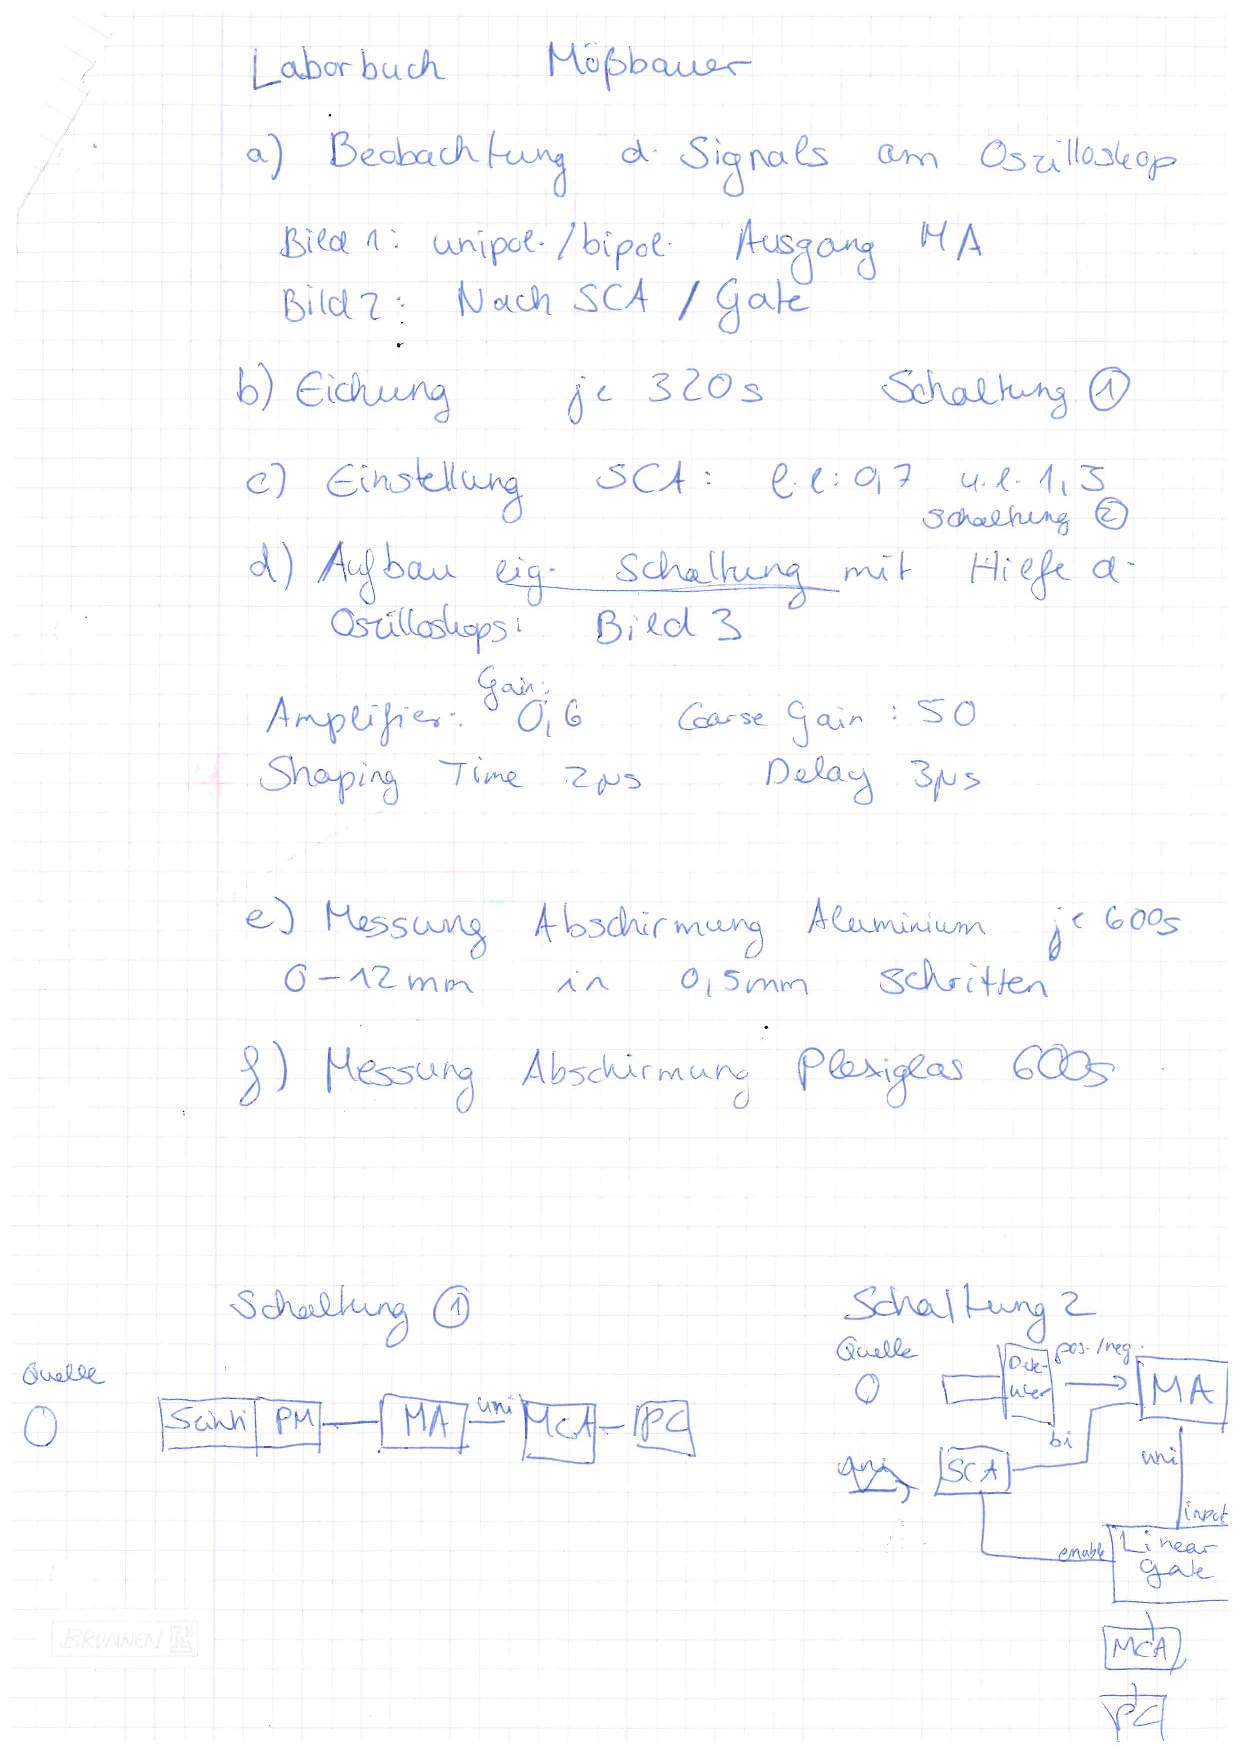
\includegraphics[width=0.9\textwidth]{../figures/laborbuch1.pdf}
\end{minipage}

\begin{minipage}{\textwidth}
	\centering
	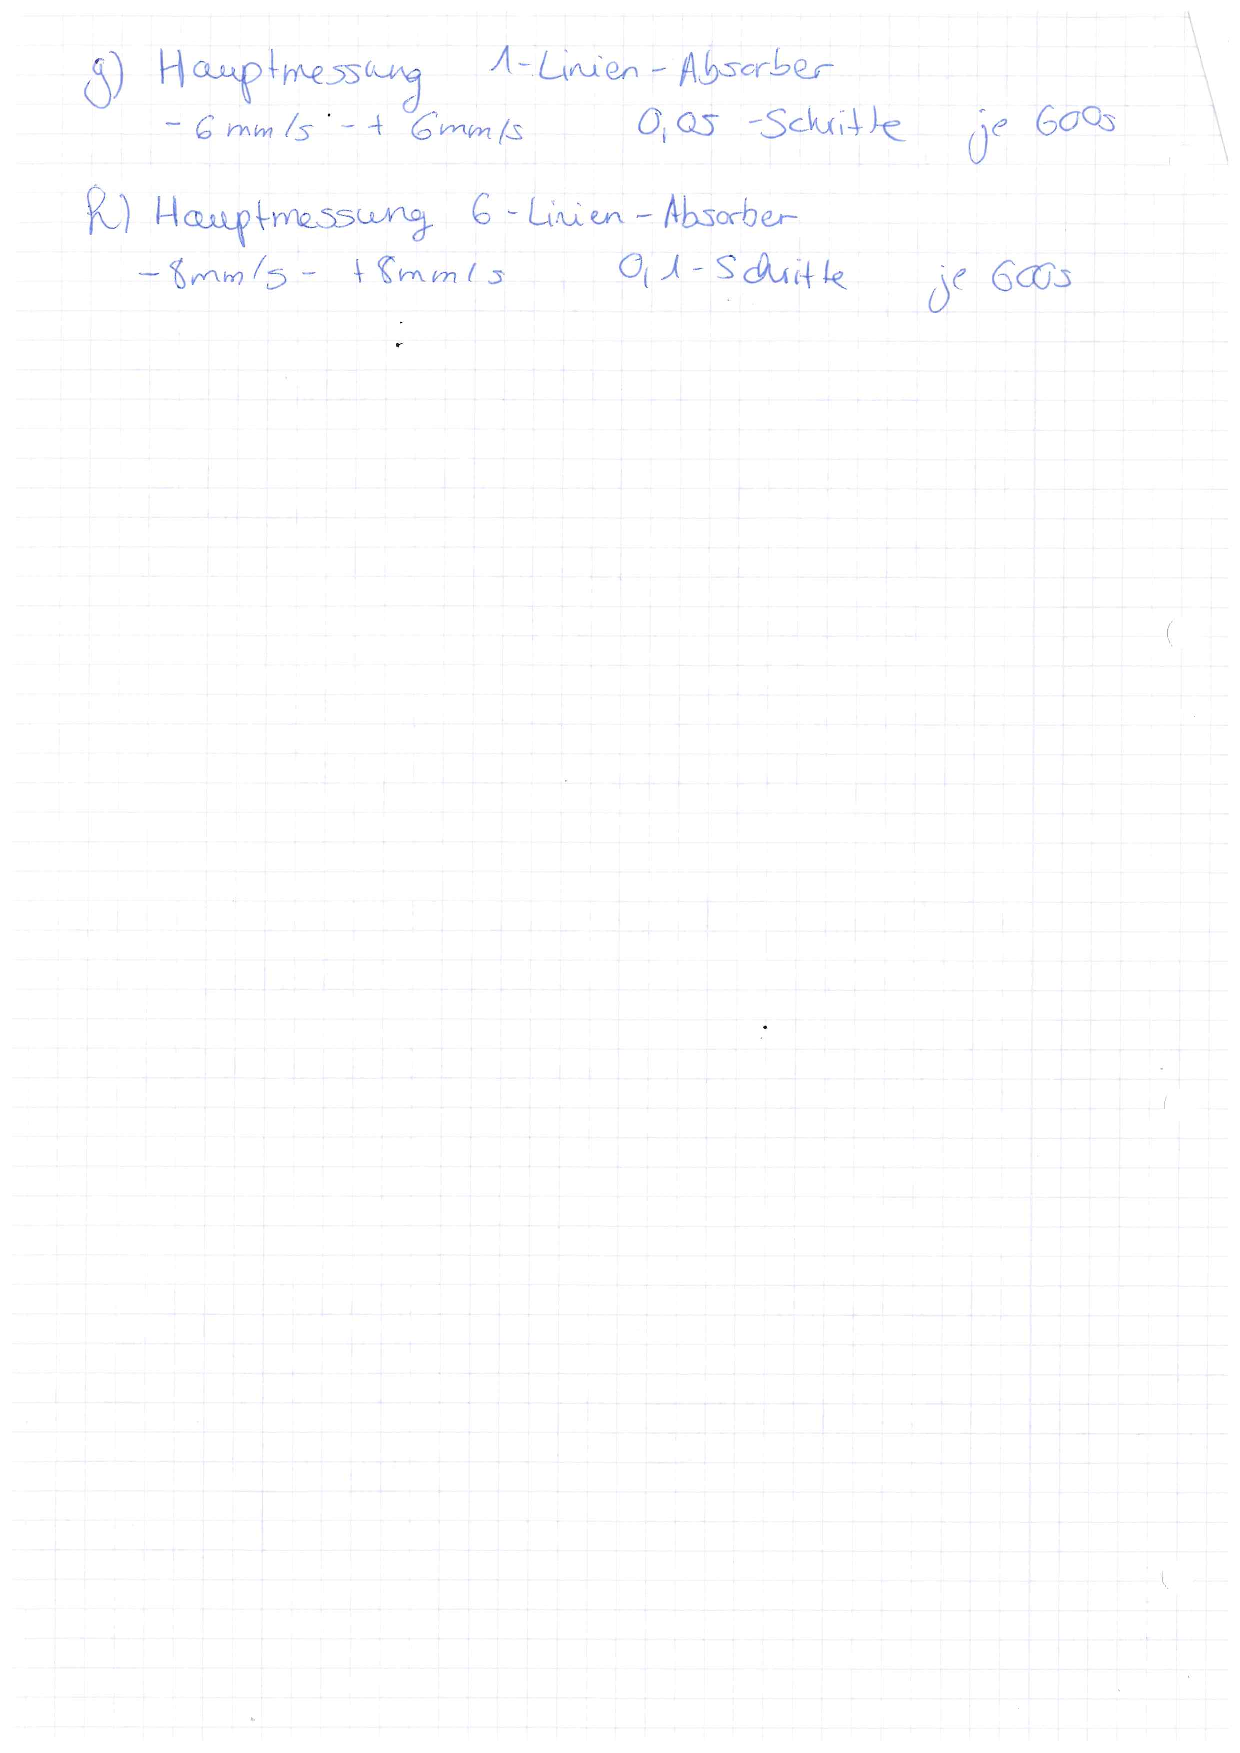
\includegraphics[width=0.9\textwidth]{../figures/laborbuch2.pdf}
\end{minipage}

\subsection{Spektren}
\label{spektren}

\subsection{Sourcecode}
\label{code}
\subsubsection*{Eichung.R}\label{Energieeichung}
\lstinputlisting[language=R]{../scripts/Eichung.R}

\subsubsection*{LinFitEichung.R}\label{LinFitEichung}
\lstinputlisting[language=R]{../scripts/LinFitEichung.R}

\subsubsection*{Compton-Untergrund.R}\label{Compton-Untergrund}
\lstinputlisting[language=R]{../scripts/aluminium.R}

\subsubsection*{Plexiglas.R}\label{Plexi}
\lstinputlisting[language=R]{../scripts/plexiglas.R}

\subsubsection*{Absorberdicke.R}\label{Absorberdicke}
\lstinputlisting[language=R]{../scripts/absorberdicke.R}

\subsubsection*{Debye-Waller.R}\label{debye}
\lstinputlisting[language=R]{../scripts/debyewaller.R}

\subsubsection*{Einlinien.R}\label{einlinien1}
\lstinputlisting[language=R]{../scripts/einlinien.R}

\subsubsection*{Sechslinien.R}\label{sechslinien}
\lstinputlisting[language=R]{../scripts/sechslinien.R}

\subsubsection*{Expfit.R}\label{exp}
\lstinputlisting[language=R]{../scripts/expfit.R}

\subsubsection*{functions.R}\label{functions}
\lstinputlisting[language=R]{../scripts/functions.R}

\subsubsection*{Gausfit.R}\label{gaus}
\lstinputlisting[language=R]{../scripts/gausfit1.R}

\subsubsection*{Lorentzfit.R}\label{lorentzfit}
\lstinputlisting[language=R]{../scripts/lorentzfit.R}

\subsubsection*{ReadFiles.R}\label{Read}
\lstinputlisting[language=R]{../scripts/readFiles.R}

\subsubsection*{Supergaus.R}\label{supergaus}
\lstinputlisting[language=R]{../scripts/supergaus.R}

\subsubsection*{Voigtfit.R}\label{voigtfit}
\lstinputlisting[language=R]{../scripts/voigtfit.R}


	\newpage
	\listoffigures
	\newpage
	\listoftables
	
	%Literatur----------------------------------------------------------------------------------------------------------
	
	%\cite{les}
	\newpage
	\printbibliography[heading=bibintoc]
	
%	\begin{thebibliography}{9}
%		
%		%\bibitem{staat}
%		%  Tobijas Kotyk,
%		%  \emph{Versuche zur Radioaktivität im Physikalischen Fortgeschrittenen Praktikum an der Albert-Ludwigs-Universität Freiburg},
%		%  Albert-Ludwigs-Universität, Freiburg,
%		%  2005
%		
%		
%		
%		%\bibitem{molmasse}
%		%  \emph{http://www.convertunits.com/molarmass/<ELEMENTNAME AUF ENGLISCH>}, Stand 28.09.2015
%		
%		
%		\bibitem{anleitung}
%		M. Köhli,
%		\emph{Versuchsanleitung Fortgeschrittenen Praktikum: SQUID},
%		Albert-Ludwigs-Universität Freiburg,
%		2011
%		
%		\bibitem{staat}
%		Volker Bange,
%		\emph{Einrichtung des Versuches "SQUID"},
%		Albert-Ludwigs-Universität Freiburg,
%		2000
%		
%		\bibitem{chemistry}
%		Bruce A. Averill, Patricia Eldredge,
%		\emph{General Chemistry: Principles, Patterns, and Applications},
%		Saylor Foundation,
%		2011
%		
%		\bibitem{SQUID}
%		Clarke, J.,
%		\emph{SQUIDS},
%		Spektrum der Wissenschaft , 10/1994,
%		Spektrum Akademischer Verlag
%	\end{thebibliography}
	
\end{document}